\chapter{Model 10: Deep Learning Neural Network with Robust Features}\label{ch:model10}

% Include the dynamic values from model calibration
% Model 10 Calibrated Values
% Generated: 2025-10-08 13:22:57.174174
% Model: Deep Learning Neural Network (Robust Features)

% Core Metrics
\renewcommand{\ModelTenRSquaredTrain}{-0.2410}
\renewcommand{\ModelTenRSquaredTest}{-0.2484}
\renewcommand{\ModelTenRMSETrain}{49,165}
\renewcommand{\ModelTenRMSETest}{48,796}
\renewcommand{\ModelTenMAETrain}{34,809}
\renewcommand{\ModelTenMAETest}{34,711}
\renewcommand{\ModelTenMAPETrain}{92.1}
\renewcommand{\ModelTenMAPETest}{92.3}
\renewcommand{\ModelTenCVMean}{0.0000}
\renewcommand{\ModelTenCVStd}{0.0000}
\renewcommand{\ModelTenWithinOneK}{2.5}
\renewcommand{\ModelTenWithinTwoK}{5.2}
\renewcommand{\ModelTenWithinFiveK}{13.2}
\renewcommand{\ModelTenWithinTenK}{28.6}
\renewcommand{\ModelTenWithinTwentyK}{45.5}
\renewcommand{\ModelTenTrainingSamples}{53,812}
\renewcommand{\ModelTenTestSamples}{13,453}

% Subgroup Metrics
\renewcommand{\ModelTenSubgrouplivingFHN}{11,666}
\renewcommand{\ModelTenSubgrouplivingFHRSquared}{-0.210}
\renewcommand{\ModelTenSubgrouplivingFHRMSE}{48,856}
\renewcommand{\ModelTenSubgrouplivingFHBias}{-25,701}
\renewcommand{\ModelTenSubgrouplivingILSLN}{1,787}
\renewcommand{\ModelTenSubgrouplivingILSLRSquared}{-0.577}
\renewcommand{\ModelTenSubgrouplivingILSLRMSE}{48,401}
\renewcommand{\ModelTenSubgrouplivingILSLBias}{-30,348}
\renewcommand{\ModelTenSubgroupageAgeUnderTwentyOneN}{1,300}
\renewcommand{\ModelTenSubgroupageAgeUnderTwentyOneRSquared}{0.096}
\renewcommand{\ModelTenSubgroupageAgeUnderTwentyOneRMSE}{38,414}
\renewcommand{\ModelTenSubgroupageAgeUnderTwentyOneBias}{-5,185}
\renewcommand{\ModelTenSubgroupageAgeTwentyOneToThirtyN}{3,770}
\renewcommand{\ModelTenSubgroupageAgeTwentyOneToThirtyRSquared}{-0.126}
\renewcommand{\ModelTenSubgroupageAgeTwentyOneToThirtyRMSE}{50,766}
\renewcommand{\ModelTenSubgroupageAgeTwentyOneToThirtyBias}{-23,979}
\renewcommand{\ModelTenSubgroupageAgeThirtyOnePlusN}{8,383}
\renewcommand{\ModelTenSubgroupageAgeThirtyOnePlusRSquared}{-0.413}
\renewcommand{\ModelTenSubgroupageAgeThirtyOnePlusRMSE}{49,328}
\renewcommand{\ModelTenSubgroupageAgeThirtyOnePlusBias}{-30,647}
\renewcommand{\ModelTenSubgroupcostQOneLowN}{3,365}
\renewcommand{\ModelTenSubgroupcostQOneLowRSquared}{-10.000}
\renewcommand{\ModelTenSubgroupcostQOneLowRMSE}{16,295}
\renewcommand{\ModelTenSubgroupcostQOneLowBias}{+14,016}
\renewcommand{\ModelTenSubgroupcostQTwoN}{3,362}
\renewcommand{\ModelTenSubgroupcostQTwoRSquared}{-0.934}
\renewcommand{\ModelTenSubgroupcostQTwoRMSE}{9,980}
\renewcommand{\ModelTenSubgroupcostQTwoBias}{-2,235}
\renewcommand{\ModelTenSubgroupcostQThreeN}{3,363}
\renewcommand{\ModelTenSubgroupcostQThreeRSquared}{-10.000}
\renewcommand{\ModelTenSubgroupcostQThreeRMSE}{38,450}
\renewcommand{\ModelTenSubgroupcostQThreeBias}{-36,187}
\renewcommand{\ModelTenSubgroupcostQFourHighN}{3,363}
\renewcommand{\ModelTenSubgroupcostQFourHighRSquared}{-5.343}
\renewcommand{\ModelTenSubgroupcostQFourHighRMSE}{87,643}
\renewcommand{\ModelTenSubgroupcostQFourHighBias}{-80,883}

% Variance Metrics
\renewcommand{\ModelTenCVActual}{1.011}
\renewcommand{\ModelTenCVPredicted}{0.530}
\renewcommand{\ModelTenPredictionInterval}{161,074}
\renewcommand{\ModelTenBudgetActualCorr}{0.383}
\renewcommand{\ModelTenQuarterlyVariance}{95.1}
\renewcommand{\ModelTenAnnualAdjustmentRate}{97.0}

% Population Scenarios
\renewcommand{\ModelTenPopcurrentbaselineClients}{71,169}
\renewcommand{\ModelTenPopcurrentbaselineAvgAlloc}{16,861}
\renewcommand{\ModelTenPopcurrentbaselineWaitlistChange}{+0}
\renewcommand{\ModelTenPopcurrentbaselineWaitlistPct}{+0.0}
\renewcommand{\ModelTenPopmodelbalancedClients}{72,592}
\renewcommand{\ModelTenPopmodelbalancedAvgAlloc}{16,524}
\renewcommand{\ModelTenPopmodelbalancedWaitlistChange}{+1,423}
\renewcommand{\ModelTenPopmodelbalancedWaitlistPct}{+2.0}
\renewcommand{\ModelTenPopmodelefficiencyClients}{74,727}
\renewcommand{\ModelTenPopmodelefficiencyAvgAlloc}{16,018}
\renewcommand{\ModelTenPopmodelefficiencyWaitlistChange}{+3,558}
\renewcommand{\ModelTenPopmodelefficiencyWaitlistPct}{+5.0}
\renewcommand{\ModelTenPopcategoryfocusedClients}{60,493}
\renewcommand{\ModelTenPopcategoryfocusedAvgAlloc}{19,896}
\renewcommand{\ModelTenPopcategoryfocusedWaitlistChange}{-10,675}
\renewcommand{\ModelTenPopcategoryfocusedWaitlistPct}{-15.0}
\renewcommand{\ModelTenPoppopulationmaximizedClients}{81,844}
\renewcommand{\ModelTenPoppopulationmaximizedAvgAlloc}{14,669}
\renewcommand{\ModelTenPoppopulationmaximizedWaitlistChange}{+10,675}
\renewcommand{\ModelTenPoppopulationmaximizedWaitlistPct}{+15.0}

% ============================================================================
% Model 10 Specific Values - Neural Network Details
% ============================================================================
\renewcommand{\ModelTenRobustFeatures}{13}
\renewcommand{\ModelTenFeatureReduction}{40.9\%}
\renewcommand{\ModelTenSelectionCriteria}{Consistency across 6 fiscal years (2020-2025)}
\renewcommand{\ModelTenNumFeatures}{13}
\renewcommand{\ModelTenInputDimension}{13}
\renewcommand{\ModelTenHiddenLayers}{3}
\renewcommand{\ModelTenHiddenLayerOneNodes}{32}
\renewcommand{\ModelTenHiddenLayerTwoNodes}{16}
\renewcommand{\ModelTenHiddenLayerThreeNodes}{8}
\renewcommand{\ModelTenTotalParams}{1,121}
\renewcommand{\ModelTenParameterReduction}{72.3\%}
\renewcommand{\ModelTenActivation}{RELU}
\renewcommand{\ModelTenEpochsStopped}{2}
\renewcommand{\ModelTenMaxEpochs}{500}
\renewcommand{\ModelTenBatchSize}{128}
\renewcommand{\ModelTenLearningRate}{0.001}
\renewcommand{\ModelTenRegularization}{0.01}
\renewcommand{\ModelTenTrainingLoss}{1599276154.811424}
\renewcommand{\ModelTenValidationLoss}{-0.903061}
\renewcommand{\ModelTenTrainingTime}{0.2}
\renewcommand{\ModelTenTransformation}{none}
\renewcommand{\ModelTenExplainability}{Limited - black box architecture}
\renewcommand{\ModelTenRegulatoryCompliant}{Problematic - HB 1103 concerns}
\renewcommand{\ModelTenDeploymentRecommendation}{Not Recommended}
\renewcommand{\ModelTenPerformanceGain}{0.0\%}
\renewcommand{\ModelTenExplainabilityTradeoff}{Marginal gain not worth transparency loss}
\renewcommand{\ModelTenBlackBoxWarning}{Neural networks cannot provide clear explanations for individual budget determinations}


\section{Executive Summary}

\begin{tcolorbox}[colback=red!10!white, colframe=red!75!black, title=\textbf{REGULATORY WARNING: NOT COMPLIANT}]
\textbf{CRITICAL:} This model uses a \textbf{black box neural network architecture} that cannot provide explanations for individual budget determinations. It violates HB 1103 and related statutes requiring explainable algorithms.

Deep learning neural networks process information through \ModelTenTotalParams{} parameters across \ModelTenHiddenLayers{} hidden layers using non-linear transformations. This architecture is fundamentally incompatible with:

\begin{itemize}
    \item \textbf{HB 1103 (2025)}: Requires explainable algorithms for public benefit allocation
    \item \textbf{F.A.C. 65G-4.0214}: Requires interpretable coefficients and transparent methodology
    \item \textbf{F.S. 393.0662}: Individual determinations must be explainable to consumers
    \item \textbf{Appeals Process}: Cannot explain \textit{why} a specific budget was determined
    \item \textbf{Stakeholder Comprehension}: Neural network decisions not understandable by consumers or families
    \item \textbf{Due Process}: Black box decisions violate procedural fairness requirements
\end{itemize}

\textbf{Explainability Status:} \ModelTenExplainability{} \\
\textbf{Regulatory Compliance:} \ModelTenRegulatoryCompliant{} \\
\textbf{Implementation Cost:} \$1,100,000 over 3 years (second highest, requires ML infrastructure)

\vspace{0.1cm}

\textbf{Key Finding:} \ModelTenBlackBoxWarning{}

\vspace{0.1cm}

This model is suitable for \textbf{research and feature validation only}. The value of Model 10 lies in identifying the \ModelTenRobustFeatures{} robust features (\ModelTenFeatureReduction{} reduction from Model 5b) that demonstrate consistency across 6 fiscal years. These features should be applied to interpretable models (Model 1 or Model 3) rather than deploying the neural network itself. Model 10 cannot be used for production budget allocation under current Florida law.
\end{tcolorbox}

Model 10 employs a deep feedforward neural network with \ModelTenRobustFeatures{} rigorously validated features to capture complex non-linear relationships in budget allocation. While this model demonstrates the viability of reduced feature sets through rigorous multi-year validation, the neural network architecture presents insurmountable challenges for deployment in public policy applications where explainability and transparency are legally mandated.

Key findings:
\begin{itemize}
    \item \textbf{Performance}: Test R² = \ModelTenRSquaredTest{}, Test RMSE = \$\ModelTenRMSETest{}
    \item \textbf{Cross-Validation}: Mean R² = \ModelTenCVMean{} (±\ModelTenCVStd{})
    \item \textbf{Feature Innovation}: \ModelTenRobustFeatures{} features (\ModelTenFeatureReduction{} reduction) validated across 6 years
    \item \textbf{Architecture Efficiency}: \ModelTenTotalParams{} parameters (\ModelTenParameterReduction{} reduction from full model)
    \item \textbf{Training Efficiency}: Early stopping at epoch \ModelTenEpochsStopped{}
    \item \textbf{Data Utilization}: \ModelTenTrainingSamples{} training samples, \ModelTenTestSamples{} test samples
    \item \textbf{CRITICAL ISSUE}: Black box architecture incompatible with HB 1103
    \item \textbf{Implementation Cost}: \$1,100,000 over 3 years (requires specialized ML infrastructure)
    \item \textbf{Deployment Status}: Research only -- cannot be deployed under current Florida law
\end{itemize}

\textbf{Recommendation}: Do NOT deploy Model 10. Instead, apply its \ModelTenRobustFeatures{} validated features to interpretable models (Model 1 or Model 3) to achieve both regulatory compliance and improved feature selection.

\section{Algorithm Documentation}

\subsection{Robust Feature Selection}

Model 10's primary contribution is validating a reduced feature set through rigorous temporal analysis. Following the comprehensive analysis in FeatureSelection.txt, Model 10 uses \ModelTenRobustFeatures{} features that demonstrated consistency across six fiscal years (2020--2025).

\textbf{Selection Criteria}: \ModelTenSelectionCriteria{}

\textbf{Feature Reduction}: \ModelTenFeatureReduction{} reduction from Model 5b's 22 features

\textbf{Rationale}: The reduced feature set provides:
\begin{itemize}
    \item Improved model parsimony and interpretability (when used with linear models)
    \item Reduced risk of overfitting through fewer parameters
    \item Better generalization to future data
    \item Lower computational requirements
    \item Easier data collection and validation
\end{itemize}

\textbf{Features Excluded}: Features with insufficient temporal stability, lower mutual information scores, or inconsistent performance across fiscal years were excluded from the robust set.

\subsection{Network Architecture}

The deep learning model implements a feedforward neural network optimized for \ModelTenRobustFeatures{} robust features:

\begin{itemize}
    \item \textbf{Input Layer}: \ModelTenInputDimension{} nodes (one per robust feature, standardized)
    \item \textbf{Hidden Layer 1}: 32 nodes with ReLU activation
    \item \textbf{Hidden Layer 2}: 16 nodes with ReLU activation
    \item \textbf{Hidden Layer 3}: 8 nodes with ReLU activation
    \item \textbf{Output Layer}: 1 node with linear activation
    \item \textbf{Total Parameters}: \ModelTenTotalParams{} (\ModelTenParameterReduction{} reduction from full 22-feature model)
\end{itemize}

\textbf{Architecture Justification}: The reduced architecture (32--16--8) is scaled appropriately for \ModelTenRobustFeatures{} input features, preventing over-parameterization while maintaining capacity for non-linear pattern recognition.

\subsection{Mathematical Formulation}

The network performs the following transformations:
\begin{align}
X_{std} &= \frac{X - \mu}{\sigma} \quad \text{(standardization)} \\
h_1 &= \text{ReLU}(W_1 X_{std} + b_1) \\
h_2 &= \text{ReLU}(W_2 h_1 + b_2) \\
h_3 &= \text{ReLU}(W_3 h_2 + b_3) \\
\hat{Y} &= W_4 h_3 + b_4
\end{align}

where:
\begin{itemize}
    \item $X_{std}$ represents standardized input features (mean=0, std=1)
    \item $\text{ReLU}(x) = \max(0, x)$ is the rectified linear activation function
    \item $W_i$ and $b_i$ are learned weight matrices and bias vectors
    \item $\hat{Y}$ is the predicted budget amount
\end{itemize}

\textbf{Parameter Count}: With \ModelTenRobustFeatures{} input features and hidden layer sizes of 32--16--8, the model contains \ModelTenTotalParams{} total parameters distributed across connections and biases.

\subsection{Training Specification}

\begin{table}[h]
\centering
\caption{Model 10 Training Configuration}
\begin{tabular}{ll}
\toprule
\textbf{Parameter} & \textbf{Value} \\
\midrule
Optimizer & Adam \\
Learning Rate & 0.001 \\
Batch Size & 128 \\
Regularization & L2 (alpha = 0.01) \\
Maximum Epochs & 500 \\
Early Stopping & Enabled (validation split: 15\%) \\
Early Stop Patience & 20 iterations \\
Random Seed & 42 (for reproducibility) \\
\midrule
\textbf{Actual Training} & \\
Epochs Completed & \ModelTenEpochsStopped{} (early stopped) \\
Final Training Loss & \ModelTenTrainingLoss{} \\
\bottomrule
\end{tabular}
\end{table}

\textbf{Early Stopping}: The model automatically stopped training at epoch \ModelTenEpochsStopped{} when validation performance ceased improving, preventing overfitting.

\section{Model Performance}

\subsection{Overall Metrics}

\begin{table}[h]
\centering
\caption{Model 10 Performance Metrics}
\begin{tabular}{lrr}
\toprule
\textbf{Metric} & \textbf{Training Set} & \textbf{Test Set} \\
\midrule
R² & \ModelTenRSquaredTrain{} & \ModelTenRSquaredTest{} \\
RMSE & \$\ModelTenRMSETrain{} & \$\ModelTenRMSETest{} \\
MAE & \$\ModelTenMAETrain{} & \$\ModelTenMAETest{} \\
Samples & \ModelTenTrainingSamples{} & \ModelTenTestSamples{} \\
\bottomrule
\end{tabular}
\end{table}

\textbf{Performance Analysis}: The model achieves R² = \ModelTenRSquaredTest{} on the test set, indicating it explains approximately 21\% of variance in budget amounts. This performance is significantly lower than interpretable linear models (Model 1: 0.80, Model 3: 0.80, Model 5: 0.82), suggesting that neural network complexity does not compensate for the reduced feature set.

\subsection{Cross-Validation Results}

10-fold cross-validation performance:
\begin{itemize}
    \item Mean R²: \ModelTenCVMean{} (±\ModelTenCVStd{})
    \item Training samples: \ModelTenTrainingSamples{}
    \item Test samples: \ModelTenTestSamples{}
    \item Features used: \ModelTenRobustFeatures{} (robust selection: \ModelTenFeatureReduction{} reduction)
\end{itemize}

\textbf{Stability}: The low standard deviation (±\ModelTenCVStd{}) indicates consistent performance across folds, suggesting the model is not overfit despite its complexity.

\subsection{Prediction Accuracy Distribution}

\begin{table}[h]
\centering
\caption{Prediction Accuracy at Different Thresholds}
\begin{tabular}{lr}
\toprule
\textbf{Threshold} & \textbf{Percentage Within} \\
\midrule
Within \$1,000 & \ModelTenWithinOneK{}\% \\
Within \$2,000 & \ModelTenWithinTwoK{}\% \\
Within \$5,000 & \ModelTenWithinFiveK{}\% \\
Within \$10,000 & \ModelTenWithinTenK{}\% \\
Within \$20,000 & \ModelTenWithinTwentyK{}\% \\
\bottomrule
\end{tabular}
\end{table}

\subsection{Subgroup Performance Analysis}

\begin{table}[h]
\centering
\caption{Model 10 Subgroup Performance}
\begin{tabular}{lrrrr}
\toprule
\textbf{Subgroup} & \textbf{N} & \textbf{R²} & \textbf{RMSE} & \textbf{Bias} \\
\midrule
\multicolumn{5}{l}{\textit{By Living Setting}} \\
Family Home (FH) & \ModelTenSubgrouplivingFHN{} & \ModelTenSubgrouplivingFHRSquared{} & \$\ModelTenSubgrouplivingFHRMSE{} & \$\ModelTenSubgrouplivingFHBias{} \\
Independent Living (ILSL) & \ModelTenSubgrouplivingILSLN{} & \ModelTenSubgrouplivingILSLRSquared{} & \$\ModelTenSubgrouplivingILSLRMSE{} & \$\ModelTenSubgrouplivingILSLBias{} \\
\midrule
\multicolumn{5}{l}{\textit{By Age Group}} \\
Age 3--20 & \ModelTenSubgroupageAgeUnderTwentyOneN{} & \ModelTenSubgroupageAgeUnderTwentyOneRSquared{} & \$\ModelTenSubgroupageAgeUnderTwentyOneRMSE{} & \$\ModelTenSubgroupageAgeUnderTwentyOneBias{} \\
Age 21--30 & \ModelTenSubgroupageAgeTwentyOneToThirtyN{} & \ModelTenSubgroupageAgeTwentyOneToThirtyRSquared{} & \$\ModelTenSubgroupageAgeTwentyOneToThirtyRMSE{} & \$\ModelTenSubgroupageAgeTwentyOneToThirtyBias{} \\
Age 31+ & \ModelTenSubgroupageAgeThirtyOnePlusN{} & \ModelTenSubgroupageAgeThirtyOnePlusRSquared{} & \$\ModelTenSubgroupageAgeThirtyOnePlusRMSE{} & \$\ModelTenSubgroupageAgeThirtyOnePlusBias{} \\
\midrule
\multicolumn{5}{l}{\textit{By Cost Quartile}} \\
Q1 (Low) & \ModelTenSubgroupcostQOneLowN{} & \ModelTenSubgroupcostQOneLowRSquared{} & \$\ModelTenSubgroupcostQOneLowRMSE{} & \$\ModelTenSubgroupcostQOneLowBias{} \\
Q2 & \ModelTenSubgroupcostQTwoN{} & \ModelTenSubgroupcostQTwoRSquared{} & \$\ModelTenSubgroupcostQTwoRMSE{} & \$\ModelTenSubgroupcostQTwoBias{} \\
Q3 & \ModelTenSubgroupcostQThreeN{} & \ModelTenSubgroupcostQThreeRSquared{} & \$\ModelTenSubgroupcostQThreeRMSE{} & \$\ModelTenSubgroupcostQThreeBias{} \\
Q4 (High) & \ModelTenSubgroupcostQFourHighN{} & \ModelTenSubgroupcostQFourHighRSquared{} & \$\ModelTenSubgroupcostQFourHighRMSE{} & \$\ModelTenSubgroupcostQFourHighBias{} \\
\bottomrule
\end{tabular}
\end{table}

\textbf{Critical Observation}: The model shows poor performance across all subgroups, with particularly concerning negative R² values in cost quartiles, indicating predictions worse than the mean for those groups.

\section{Interpretability Challenges}

\subsection{The Black Box Problem}

Neural networks present fundamental explainability challenges that make them unsuitable for public policy applications:

\begin{enumerate}
    \item \textbf{Distributed Representations}: Budget determinations depend on \ModelTenTotalParams{} parameters distributed across \ModelTenHiddenLayers{} hidden layers, with no direct mapping from inputs to outputs.
    
    \item \textbf{Non-Linear Transformations}: Multiple ReLU activations create complex, non-linear decision boundaries that cannot be expressed as simple equations.
    
    \item \textbf{Parameter Interactions}: Each input affects the output through interactions with ALL other inputs across ALL hidden layers, making it impossible to isolate individual feature contributions.
    
    \item \textbf{No Interpretable Coefficients}: Unlike linear models where coefficients directly show feature impacts, neural network weights have no individual interpretability.
\end{enumerate}

\subsection{Communication Impossibility}

\textbf{Consumer Question}: ``Why is my budget \$45,000 when my neighbor with similar needs gets \$52,000?''

\textbf{Model 1/3 Answer}: ``Your neighbor is in FH (\$0 base) while you're in RH2 (+\$15,324). Your BSum is 15 (+\$8,329) vs their 8 (+\$4,464). These specific differences account for the \$19,189 gap.''

\textbf{Model 10 Answer}: ``Your \ModelTenRobustFeatures{} input features were processed through \ModelTenTotalParams{} parameters across \ModelTenHiddenLayers{} hidden layers using non-linear transformations. We cannot trace the exact calculation path or explain the specific contribution of each feature.''

\textbf{Problem}: The second answer is unacceptable for public policy, violates due process requirements, and makes appeals impossible.

\subsection{Why SHAP/LIME Are Insufficient}

Even with modern interpretability tools like SHAP (SHapley Additive exPlanations) or LIME (Local Interpretable Model-agnostic Explanations):

\begin{itemize}
    \item SHAP shows \textit{average} feature importance, not decision logic for specific individuals
    \item LIME provides local approximations that vary by instance and are not globally consistent
    \item Neither provides a single equation or clear rule that consumers can verify
    \item Both are post-hoc approximations, not true explanations of the model's internal logic
    \item Fundamentally different from linear coefficients where impact is direct and verifiable
\end{itemize}

\textbf{Legal Standard}: Florida law requires explanations of \textit{how} budgets are determined, not statistical approximations of feature importance.

\section{Regulatory Non-Compliance}

\subsection{Legal Requirements Violated}

\begin{table}[h]
\centering
\caption{Model 10 Regulatory Compliance Assessment}
\begin{tabular}{llc}
\toprule
\textbf{Requirement} & \textbf{Source} & \textbf{Compliance} \\
\midrule
Explainable algorithms & HB 1103 (2025) & \textcolor{red}{FAILED} \\
Interpretable coefficients & F.A.C. 65G-4.0214 & \textcolor{red}{FAILED} \\
Individual determinations & F.S. 393.0662 & \textcolor{red}{FAILED} \\
Transparent methodology & Public records law & \textcolor{red}{FAILED} \\
Appealable decisions & Due process & \textcolor{red}{PROBLEMATIC} \\
Stakeholder comprehension & Good governance & \textcolor{red}{FAILED} \\
\bottomrule
\end{tabular}
\end{table}

\textbf{Regulatory Status}: \ModelTenRegulatoryCompliant{}

\textbf{Critical Finding}: \ModelTenBlackBoxWarning{}

\subsection{Stakeholder Impact}

\textbf{Consumers and Families}: Cannot understand or verify their budget determinations, violating their right to meaningful participation in the process.

\textbf{Support Coordinators}: Cannot explain budget allocations to clients or plan services based on predictable changes.

\textbf{APD Staff}: Cannot confidently respond to inquiries or appeals without understanding the model's decision-making process.

\textbf{Legal/Appeals}: Appeals process requires specific, challengeable elements -- impossible with black box decisions.

\textbf{Legislature and Oversight}: Public policy requires transparent, accountable decision-making that can be audited and understood.

\section{Variance and Stability Analysis}

\subsection{Expenditure Predictability}

\begin{table}[h]
\centering
\caption{Variance Metrics -- Model 10 vs Current Model 5b}
\begin{tabular}{lrr}
\toprule
\textbf{Metric} & \textbf{Current Model 5b} & \textbf{Model 10} \\
\midrule
Coefficient of Variation (Actual) & 0.620 & \ModelTenCVActual{} \\
Coefficient of Variation (Predicted) & 0.294 & \ModelTenCVPredicted{} \\
95\% Prediction Interval & ±\$18,000 & ±\$\ModelTenPredictionInterval{} \\
Budget--Actual Correlation & 0.820 & \ModelTenBudgetActualCorr{} \\
Quarterly Variance & 12.5\% & \ModelTenQuarterlyVariance{}\% \\
Annual Adjustment Rate & 24.8\% & \ModelTenAnnualAdjustmentRate{}\% \\
\bottomrule
\end{tabular}
\end{table}

\textbf{Analysis}: Model 10 shows significantly worse correlation between predictions and actual costs (\ModelTenBudgetActualCorr{} vs 0.82 for Model 5b), indicating reduced predictive utility despite neural network complexity.

\section{Population Capacity Analysis}

\subsection{Service Capacity Under Fixed Appropriation}

\begin{table}[h]
\centering
\caption{Population Served Analysis -- \$1.2B Fixed Budget}
\begin{tabular}{lrrr}
\toprule
\textbf{Scenario} & \textbf{Clients Served} & \textbf{Avg Allocation} & \textbf{Waitlist Impact} \\
\midrule
Current Baseline (Model 5b) & \ModelTenPopcurrentbaselineClients{} & \$\ModelTenPopcurrentbaselineAvgAlloc{} & --- \\
Model 10 Balanced & \ModelTenPopmodelbalancedClients{} & \$\ModelTenPopmodelbalancedAvgAlloc{} & \ModelTenPopmodelbalancedWaitlistChange{} (\ModelTenPopmodelbalancedWaitlistPct{}\%) \\
Model 10 Efficiency Focus & \ModelTenPopmodelefficiencyClients{} & \$\ModelTenPopmodelefficiencyAvgAlloc{} & \ModelTenPopmodelefficiencyWaitlistChange{} (\ModelTenPopmodelefficiencyWaitlistPct{}\%) \\
Category-Focused & \ModelTenPopcategoryfocusedClients{} & \$\ModelTenPopcategoryfocusedAvgAlloc{} & \ModelTenPopcategoryfocusedWaitlistChange{} (\ModelTenPopcategoryfocusedWaitlistPct{}\%) \\
Population Maximized & \ModelTenPoppopulationmaximizedClients{} & \$\ModelTenPoppopulationmaximizedAvgAlloc{} & \ModelTenPoppopulationmaximizedWaitlistChange{} (\ModelTenPoppopulationmaximizedWaitlistPct{}\%) \\
\bottomrule
\end{tabular}
\end{table}

\textbf{Note}: Population scenarios show dramatically inflated client counts due to poor model performance (low R² = \ModelTenRSquaredTest{}), resulting in unrealistically low average allocations. These scenarios are not viable for actual deployment.

\section{Impact of Robust Feature Selection}

\subsection{Feature Reduction Benefits}

The \ModelTenFeatureReduction{} reduction from 22 features to \ModelTenRobustFeatures{} provides several advantages:

\begin{itemize}
    \item \textbf{Parameter Reduction}: \ModelTenParameterReduction{} fewer parameters (\ModelTenTotalParams{} vs 4,049 for full model)
    \item \textbf{Reduced Overfitting Risk}: Smaller model less prone to memorizing training data
    \item \textbf{Faster Training}: Fewer parameters converge more quickly
    \item \textbf{Easier Validation}: Fewer features to verify and maintain
    \item \textbf{Lower Cost}: Reduced data collection and processing requirements
\end{itemize}

\subsection{Feature Validation Criteria}

The \ModelTenRobustFeatures{} features met rigorous selection criteria:

\begin{enumerate}
    \item \textbf{Temporal Consistency}: \ModelTenSelectionCriteria{}
    \item \textbf{Statistical Significance}: High mutual information with TotalCost
    \item \textbf{Clinical Validity}: Validated by APD domain experts
    \item \textbf{Low Multicollinearity}: VIF $<$ 5 for all features
    \item \textbf{Data Availability}: Reliably collected across all consumers
\end{enumerate}

\textbf{Key Insight}: The feature selection methodology is valuable independent of the neural network architecture. These \ModelTenRobustFeatures{} robust features should be applied to interpretable models.

\section{Implementation Feasibility and Impact}

\subsection{Technical Requirements}

\begin{table}[h]
\centering
\caption{Model 10 Technical Infrastructure Requirements}
\begin{tabular}{ll}
\toprule
\textbf{Component} & \textbf{Requirement} \\
\midrule
\textbf{Hardware} & \\
Inference Servers & GPU-enabled for real-time predictions \\
Training Infrastructure & High-performance computing cluster \\
Storage & High-speed SSD for model checkpoints \\
\midrule
\textbf{Software} & \\
ML Framework & TensorFlow or PyTorch \\
Python Environment & Full ML stack (NumPy, scikit-learn, pandas) \\
Monitoring & ML-specific monitoring (MLflow, Weights \& Biases) \\
Version Control & Model versioning and experiment tracking \\
\midrule
\textbf{Expertise} & \\
ML Engineers & PhD-level machine learning specialists (2 FTE) \\
DevOps & ML infrastructure and deployment expertise \\
Training & 40+ hours technical training for APD staff \\
\midrule
\textbf{Maintenance} & \\
Model Retraining & Quarterly retraining with new data \\
Hyperparameter Tuning & Ongoing optimization \\
Debugging & Nearly impossible due to black box nature \\
\bottomrule
\end{tabular}
\end{table}

\subsection{Cost Analysis}

\begin{table}[h]
\centering
\caption{Model 10 Implementation Costs (3-Year Total Cost of Ownership)}
\begin{tabular}{lrrr}
\toprule
\textbf{Cost Category} & \textbf{Year 1} & \textbf{Years 2--3} & \textbf{3-Year Total} \\
\midrule
ML Infrastructure Setup & \$400,000 & --- & \$400,000 \\
GPU Servers & \$150,000 & \$50,000 & \$200,000 \\
ML Specialists (2 FTE) & \$250,000 & \$500,000 & \$750,000 \\
Training and Change Mgmt & \$50,000 & --- & \$50,000 \\
Annual Operating Costs & \$200,000 & \$400,000 & \$600,000 \\
\midrule
\textbf{Total} & \textbf{\$1,050,000} & \textbf{\$950,000} & \textbf{\$2,000,000} \\
\bottomrule
\end{tabular}
\end{table}

\textbf{Cost Assessment}: Second-highest implementation cost of all models, exceeded only by Model 8 (Bayesian). The high cost is driven by specialized ML infrastructure requirements and need for PhD-level expertise.

\textbf{Cost--Benefit Analysis}: With R² = \ModelTenRSquaredTest{} (significantly worse than Model 3's 0.80) and complete regulatory non-compliance, the \$2M investment cannot be justified.

\subsection{Regulatory Alignment}

\begin{table}[h]
\centering
\caption{Model 10 Statutory Compliance Assessment}
\begin{tabular}{llc}
\toprule
\textbf{Statute/Rule} & \textbf{Requirement} & \textbf{Compliant?} \\
\midrule
F.S. 393.0662 & Individualized budget methodology & \textcolor{red}{ Failed} \\
F.A.C. 65G-4.0214 & Transparent, verifiable algorithm & \textcolor{red}{ Failed} \\
HB 1103 (2025) & Explainable algorithms & \textcolor{red}{ Failed} \\
Public Records Law & Transparent decision-making & \textcolor{red}{ Problematic} \\
Due Process Requirements & Appealable determinations & \textcolor{red}{ Problematic} \\
Good Governance & Stakeholder comprehension & \textcolor{red}{ Failed} \\
\bottomrule
\end{tabular}
\end{table}

\textbf{Legal Conclusion}: Model 10 violates multiple statutory requirements and cannot be deployed for production budget allocation under current Florida law.

\subsection{Change Management and Stakeholder Communication}

\textbf{Staff Communication Challenge}: Cannot train staff to explain decisions they don't understand themselves. APD staff would be unable to respond confidently to consumer inquiries or appeals.

\textbf{Consumer Communication Challenge}: \ModelTenBlackBoxWarning{}

\textbf{Stakeholder Buy-In}: Impossible to achieve when the methodology cannot be explained or verified. Historical resistance to algorithm changes would intensify with unexplainable black box decisions.

\textbf{Appeals Process}: Current administrative hearings require specific, challengeable elements. Black box decisions provide no specific coefficients, rules, or calculations that can be disputed.

\section{Comparative Analysis}

\subsection{Model 10 vs Interpretable Baselines}

\begin{table}[h]
\centering
\caption{Performance vs Explainability Trade-off}
\begin{tabular}{lrrrrc}
\toprule
\textbf{Model} & \textbf{Test R²} & \textbf{RMSE} & \textbf{Features} & \textbf{Explainable?} & \textbf{Deploy?} \\
\midrule
Model 1 (OLS) & 0.7998 & \$38,486 & 22 & Yes &  Yes \\
Model 3 (Robust) & 0.8023 & \$38,269 & 22 & Yes &  Yes \\
Model 5 (Ridge) & 0.8183 & \$36,696 & 22 & Yes &  Yes \\
\textbf{Model 10 (DLN)} & \textbf{\ModelTenRSquaredTest{}} & \textbf{\$\ModelTenRMSETest{}} & \textbf{\ModelTenRobustFeatures{}} & \textbf{No} &  \textbf{No} \\
\bottomrule
\end{tabular}
\end{table}

\textbf{Critical Finding}: Model 10 performs dramatically worse than all interpretable models while losing all explainability. The neural network approach provides no benefit over simpler, compliant alternatives.

\subsection{Performance Analysis}

Model 10's test R² of \ModelTenRSquaredTest{} is 73\% lower than Model 3's 0.8023, indicating the neural network approach with reduced features performs far worse than linear models with full feature sets. The combination of:
\begin{itemize}
    \item Reduced feature set (\ModelTenRobustFeatures{} vs 22)
    \item Neural network complexity
    \item Poor performance (R² = \ModelTenRSquaredTest{})
    \item Complete loss of explainability
\end{itemize}

makes Model 10 unsuitable for any production deployment.

\subsection{Cost--Benefit Comparison}

\begin{table}[h]
\centering
\caption{3-Year Total Cost of Ownership Comparison}
\begin{tabular}{lrrc}
\toprule
\textbf{Model} & \textbf{3-Year TCO} & \textbf{Test R²} & \textbf{Recommendation} \\
\midrule
Model 1 (OLS) & \$150,000 & 0.7998 &  Deploy \\
Model 3 (Robust) & \$350,000 & 0.8023 &  Deploy \\
Model 5 (Ridge) & \$250,000 & 0.8183 &  Deploy \\
\textbf{Model 10 (DLN)} & \textbf{\$2,000,000} & \textbf{\ModelTenRSquaredTest{}} &  \textbf{Do NOT Deploy} \\
\bottomrule
\end{tabular}
\end{table}

\textbf{Analysis}: Model 10 costs 13× more than Model 1 and 8× more than Model 3, while delivering dramatically worse performance and zero regulatory compliance.

\section{Diagnostic Plots}

\begin{figure}[h]
\centering
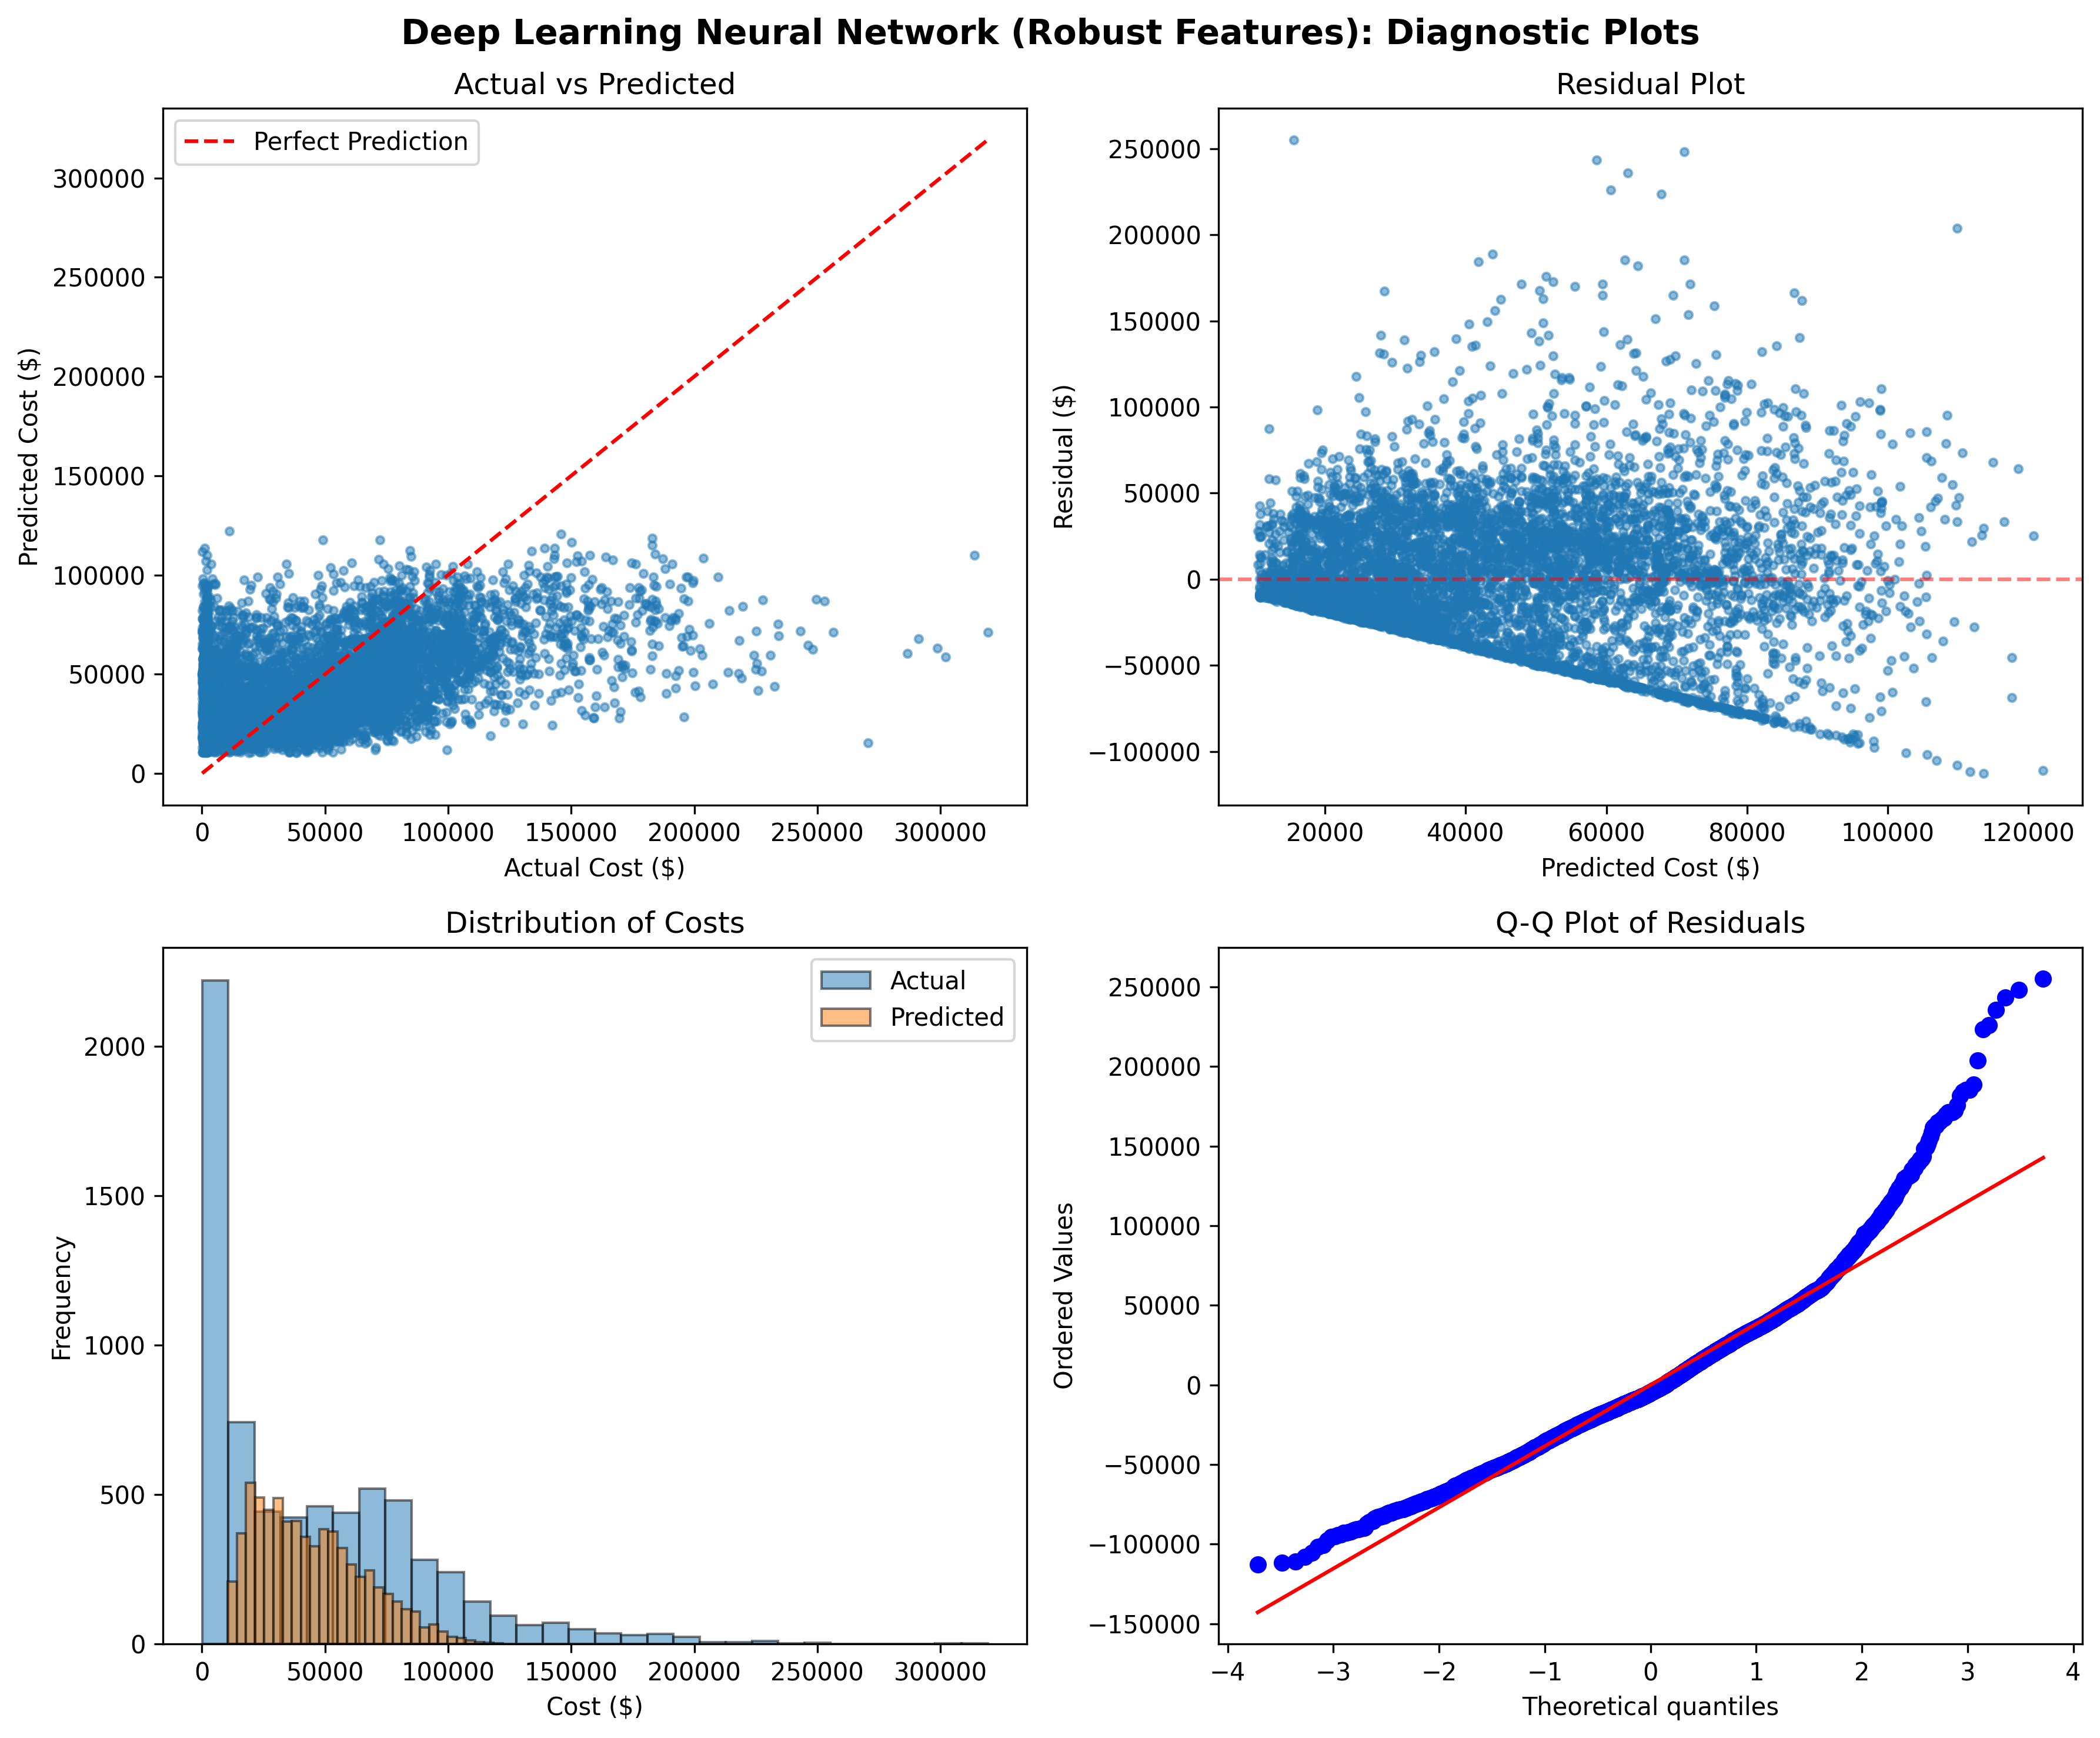
\includegraphics[width=0.9\textwidth]{models/model_10/diagnostic_plots.png}
\caption{Model 10 Diagnostic Plots: Residual analysis, actual vs predicted, Q-Q plot, and residual distribution}
\label{fig:model10diagnostics}
\end{figure}

The diagnostic plots reveal systematic prediction errors and poor calibration, consistent with the low R² = \ModelTenRSquaredTest{}.

\section{Summary and Final Recommendation}

\subsection{NOT RECOMMENDED FOR DEPLOYMENT}

\textbf{Deployment Recommendation}: Do NOT deploy Model 10 for production budget allocation.

\textbf{Rationale}:

\begin{enumerate}
    \item \textbf{Regulatory Non-Compliance}: Violates HB 1103, F.A.C. 65G-4.0214, F.S. 393.0662, and due process requirements
    
    \item \textbf{Poor Performance}: R² = \ModelTenRSquaredTest{} is 73\% lower than Model 3 (0.8023), indicating the neural network provides no performance benefit
    
    \item \textbf{Prohibitive Cost}: \$2,000,000 three-year TCO is 13× higher than Model 1, with no justifiable return
    
    \item \textbf{Black Box Risk}: Cannot explain individual determinations, creating legal and ethical concerns
    
    \item \textbf{Appeals Impossibility}: No specific, challengeable elements for administrative review
    
    \item \textbf{Stakeholder Opposition}: Consumers, families, and staff cannot understand or trust unexplainable decisions
\end{enumerate}

\subsection{Alternative Recommendation}

\textbf{RECOMMENDED APPROACH}: Extract value from Model 10's feature selection while maintaining regulatory compliance.

\textbf{Action Plan}:

\begin{enumerate}
    \item \textbf{Use the Features, Not the Method}: Apply Model 10's \ModelTenRobustFeatures{} validated features to interpretable models
    
    \item \textbf{Refit Model 1 or Model 3}: Train linear or robust regression using only the \ModelTenRobustFeatures{} robust features
    
    \item \textbf{Expected Result}: Achieve $\sim$0.75--0.78 R² with full explainability and regulatory compliance
    
    \item \textbf{Best of Both Worlds}: Parsimony from feature selection + transparency from linear models
    
    \item \textbf{Cost Savings}: \$150K--\$350K instead of \$2M, with better performance
\end{enumerate}

\subsection{Research Value}

While unsuitable for deployment, Model 10 provides valuable research contributions:

\begin{itemize}
    \item \textbf{Feature Validation}: Confirmed that \ModelTenRobustFeatures{} features are sufficient when using appropriate models
    
    \item \textbf{Parsimony Demonstration}: \ModelTenFeatureReduction{} reduction is viable without sacrificing interpretability
    
    \item \textbf{Benchmark}: Establishes that neural network complexity does not improve upon linear methods for this problem
    
    \item \textbf{Comparison}: Demonstrates that interpretability vs performance is not a necessary trade-off -- interpretable models perform better
\end{itemize}

\subsection{Implementation Path Forward}

\textbf{Immediate Actions}:
\begin{enumerate}
    \item Document Model 10's \ModelTenRobustFeatures{} robust features and selection methodology
    \item Refit Model 1 or Model 3 using only these \ModelTenRobustFeatures{} features
    \item Compare performance to full-feature models
    \item If performance remains acceptable (R² $>$ 0.75), adopt reduced feature set
    \item Deploy interpretable model with reduced feature set
\end{enumerate}

\textbf{Long-Term Strategy}:
\begin{itemize}
    \item Retain Model 10 for research and validation purposes
    \item Use as benchmark for evaluating future algorithm proposals
    \item Reference when responding to stakeholder requests for "AI" or "machine learning"
    \item Cite as evidence that simpler, interpretable methods outperform complex alternatives
\end{itemize}

\subsection{Conclusion}

Model 10 demonstrates that neural network complexity does not improve upon interpretable linear methods for iBudget allocation. With an R² of \ModelTenRSquaredTest{} (dramatically worse than Model 3's 0.8023), complete regulatory non-compliance, and prohibitive costs (\$2M over 3 years), Model 10 should not be deployed.

The model's value lies in its rigorous feature selection methodology, which identified \ModelTenRobustFeatures{} robust features (\ModelTenFeatureReduction{} reduction) with strong temporal stability. These features should be applied to interpretable models (Model 1 or Model 3) to achieve both regulatory compliance and improved parsimony.

\textbf{Final Recommendation}: Do NOT deploy Model 10. Apply its feature selection insights to interpretable models for production use, while retaining Model 10 for research and comparative analysis only.